\documentclass[a4paper, 11pt]{article}

\usepackage[utf8]{inputenc}
\usepackage[english]{babel}

\usepackage{hyperref}

\usepackage{graphicx}
\usepackage{float}

\usepackage{listings}
\usepackage{xcolor}
\definecolor{listinggray}{gray}{0.9}
\definecolor{lbcolor}{rgb}{0.9,0.9,0.9}
\lstset{
	backgroundcolor=\color{lbcolor},
	tabsize=4,    
	language=[GNU]C++,
	basicstyle=\scriptsize,
	upquote=true,
	aboveskip={1.5\baselineskip},
	columns=fixed,
	showstringspaces=false,
	extendedchars=false,
	breaklines=true,
	prebreak = \raisebox{0ex}[0ex][0ex]{\ensuremath{\hookleftarrow}},
	frame=single,
	numbers=left,
	showtabs=false,
	showspaces=false,
	showstringspaces=false,
	identifierstyle=\ttfamily,
	keywordstyle=\color[rgb]{0,0,1},
	commentstyle=\color[rgb]{0.026,0.112,0.095},
	stringstyle=\color[rgb]{0.627,0.126,0.941},
	numberstyle=\color[rgb]{0.205, 0.142, 0.73},
}

\lstset{
	backgroundcolor=\color{lbcolor},
	tabsize=4,
	language=C++,
	captionpos=b,
	tabsize=3,
	frame=lines,
	numbers=left,
	numberstyle=\tiny,
	numbersep=5pt,
	breaklines=true,
	showstringspaces=false,
	basicstyle=\footnotesize,
	%  identifierstyle=\color{magenta},
	keywordstyle=\color[rgb]{0,0,1},
	commentstyle=\color{Darkgreen},
	stringstyle=\color{red}
}

\usepackage{fullpage}

\begin{document}
	\begin{centering}
		\large\textbf{Progress Report: 05/04/2017}\\
		~\\
		Oussama ENNAFII:
		\normalsize MATIS | TITANE \\
		Directors: Cl\'ement Mallet \& Florent Lafarge \\
		Advisor: Arnaud Le Bris \\		
	\end{centering} 


	\section*{Data:}
	
	\begin{itemize}
		\item I am concentrating on Elancourt right now:
		\begin{itemize}
			\item[-] The area encompasses an industrial area with shoe box buildings, a residential area with a lot of building similarities and a very sparse urban areas;
			\item[-] I have every data possible on the area: DSM, 3D building models and Orthoimages.
		\end{itemize}
	\end{itemize}
	
	\section*{Implementation:}
	Implementation status:
	\begin{itemize}
		\item Implemented:
			\begin{itemize}
				\item[-] Reader: 3DS and OFF,
				\item[-] Geomview viewer;
				\item[-] Automated testing;
				\item[-] Algorithms on bricks: area, contour length, affine transformations;
				\item[-] Project 3D models in 2D;
				\item[-] Occlusion management.
				\item[-] Save projections into georeferenced vectorial images using GDAL;
				\item[-] Rasterize projections for DSM comparison;
				\item[-] Save raster projections into georeferenced images using GDAL;
				\item[-] Stitch Meshes (in order to stitch rooftops to facets);
				\item[-] Read Scene tree from XML file.
				\item[-] Imporved grately rasterization: with no artifacts, pixel size $= 6 cm $ $\Rightarrow$ all  Elancourt in one day.
			\end{itemize}
		\item To add:
			\begin{itemize}
				\item[-] Project 3D model on Camera.
		\end{itemize}
		\item To complete:
			\begin{itemize}
				\item[-] Improve logging.
			\end{itemize}
	\end{itemize}
	
	\begin{figure}[H]
		\caption{\label{diag::class} New changes to the program architecture.}
		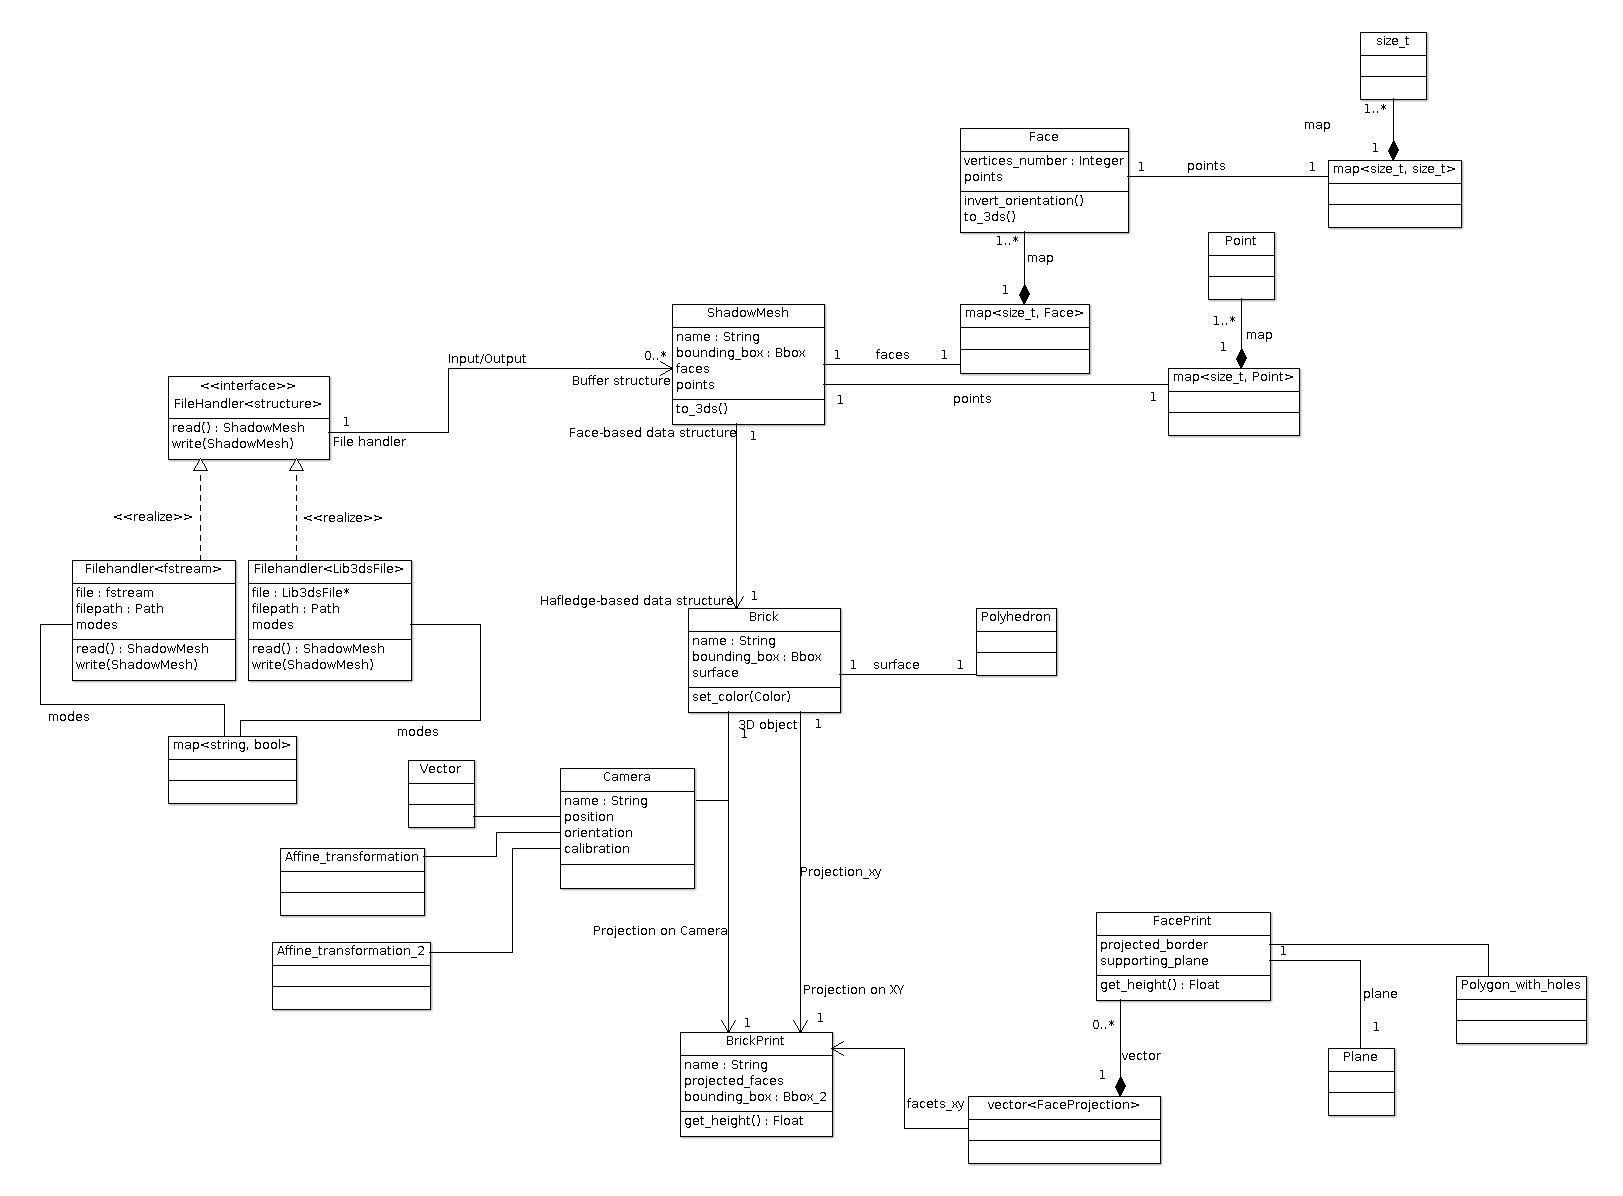
\includegraphics[scale=.27]{images/vectorial/class_diagram.png}
	\end{figure}
	
	\section*{Ideas:}
	I have identified two possible approaches in mind:
	\begin{itemize}
		\item[-] DSM and Z profil local comparison:
		\begin{itemize}
			\item[-] Simple Thresholding for inexistant buildings that are reconstructed with terrain height.
			\item[-] The difference still has structure - we can still see the facet borders - $\Rightarrow$ we can use the distribution of the difference (texture)  in order to determine if is noise or if the reconstruction missed something.
		\end{itemize}
		\item[-] Global building autoqualification:
		\begin{itemize}
			\item[-] Computed dual graph of each roof. Possibility of a bag of Features approach to get the similarity in neighborhoods.
		\end{itemize}
		
		\item[-] Orthoimage comparison:
		\begin{itemize}
			\item[-] Compute gradients "along" of building prints in order to detect any difference between inside or outside a facet/ building.
		\end{itemize}
	\end{itemize}
	
	\section*{Results:}
	\begin{figure}[H]
		\begin{center}
			\caption{\label{img::comparison} Example of building Z profile and its comparison with DSM: from left to right, up to bottom, the z profile, the  masked dsm , the laplacian of the difference, the orientation of the difference gradients, the amplitude of the difference gradient and the histogram corresponding to the orientations of the difference gradients.}
			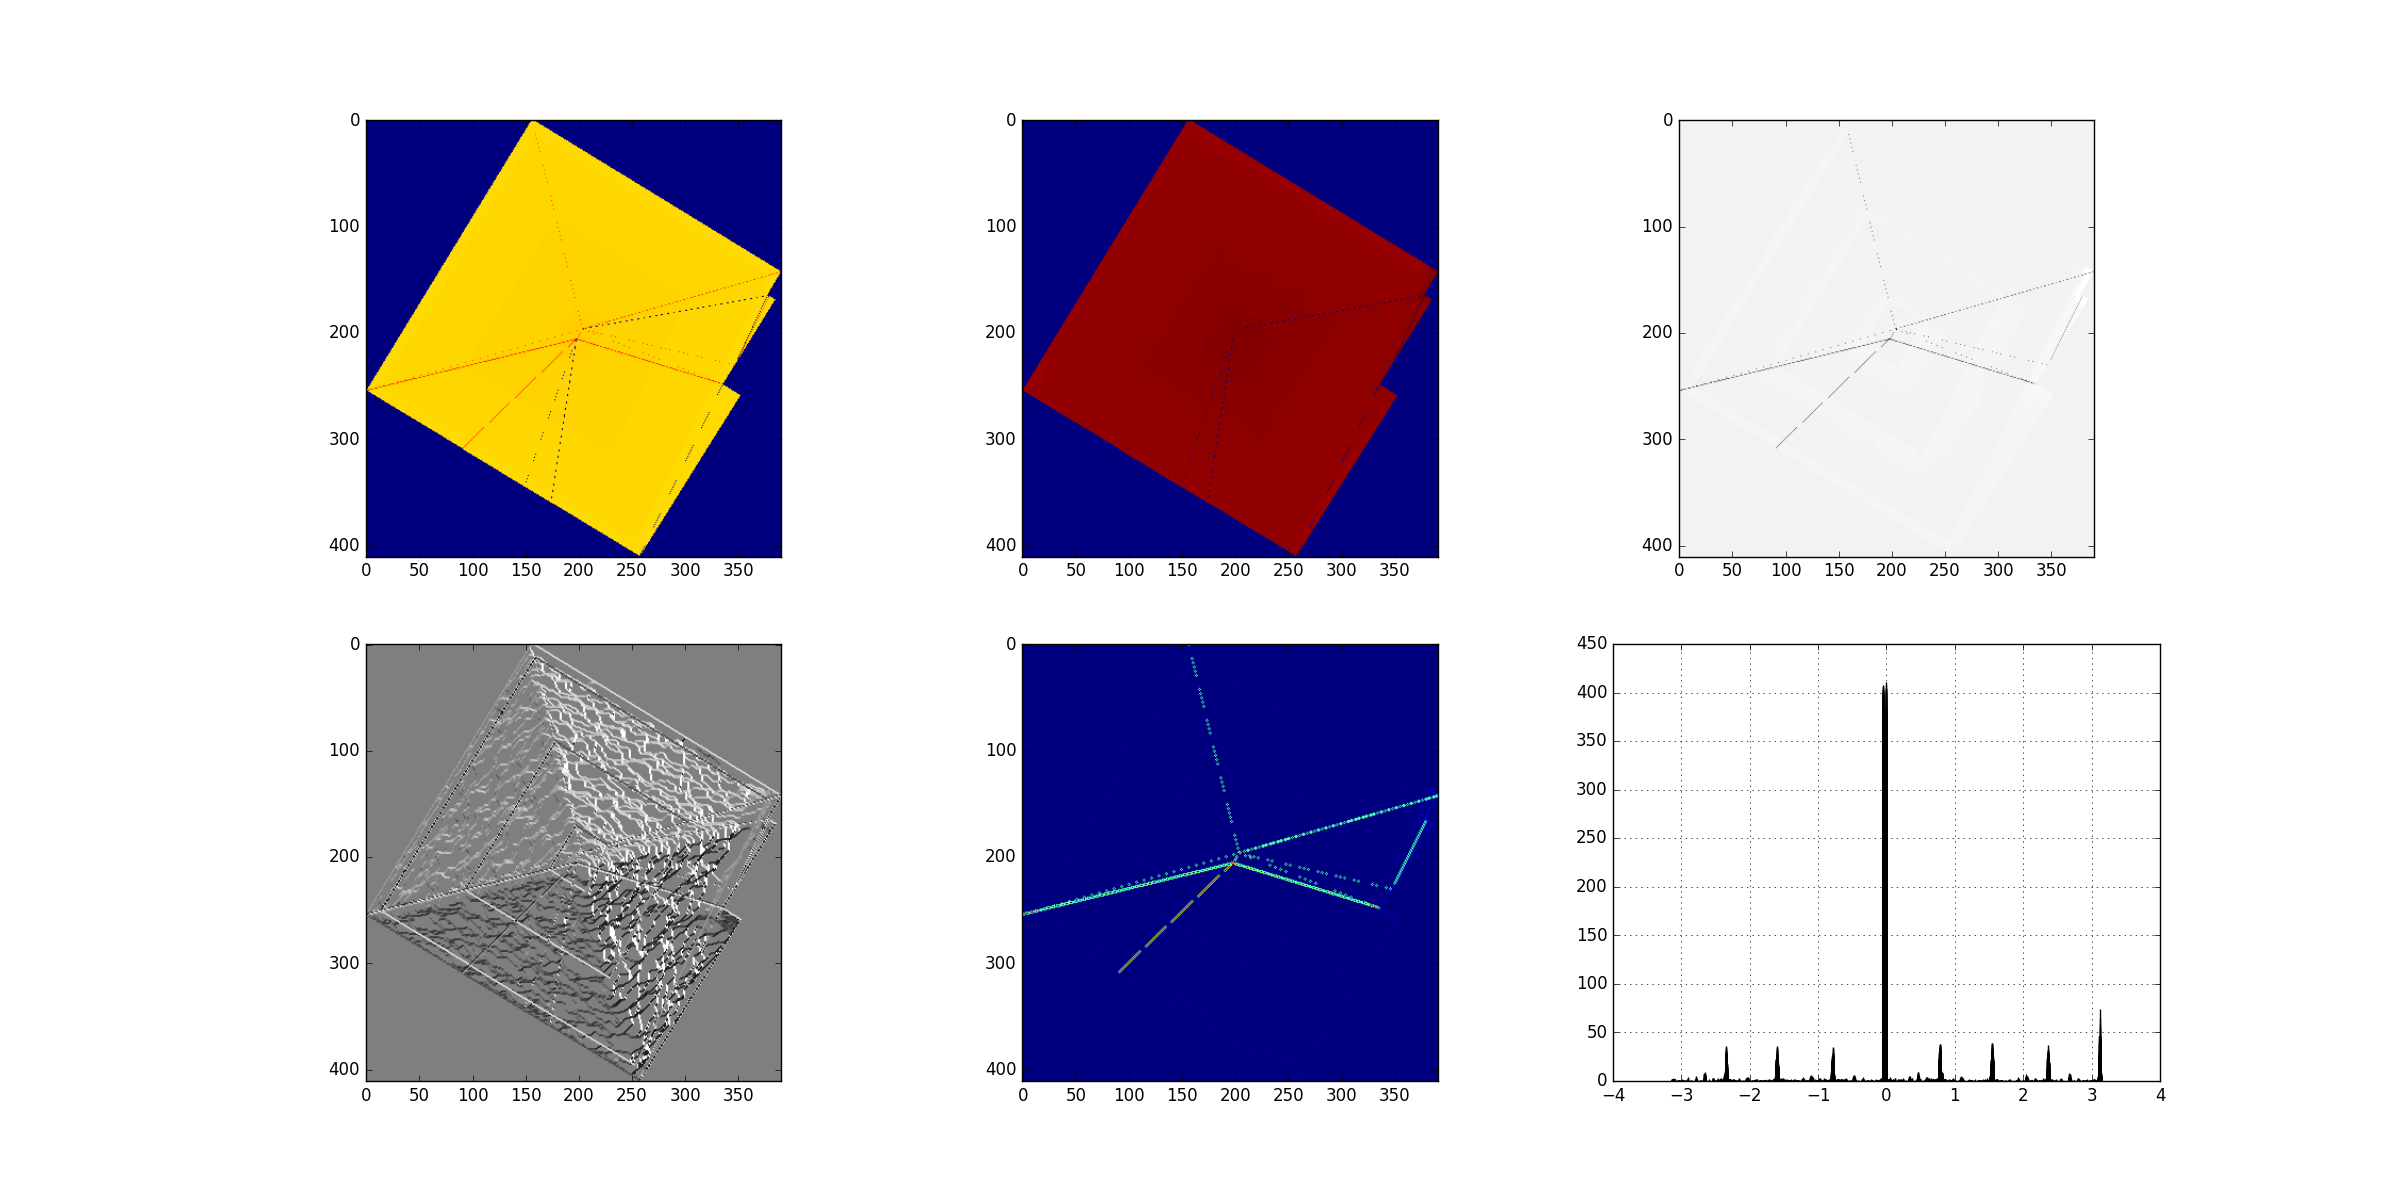
\includegraphics[scale=.25]{images/raster/elancourt/prototyping_1246-13704_T25177_T25178_T25179_T25180.png}
		\end{center}
	\end{figure}
	
	\begin{figure}[H]
		\begin{center}
			\caption{\label{img::comparison_bis} The same comparison applied for a building with chimney (not visible).}
			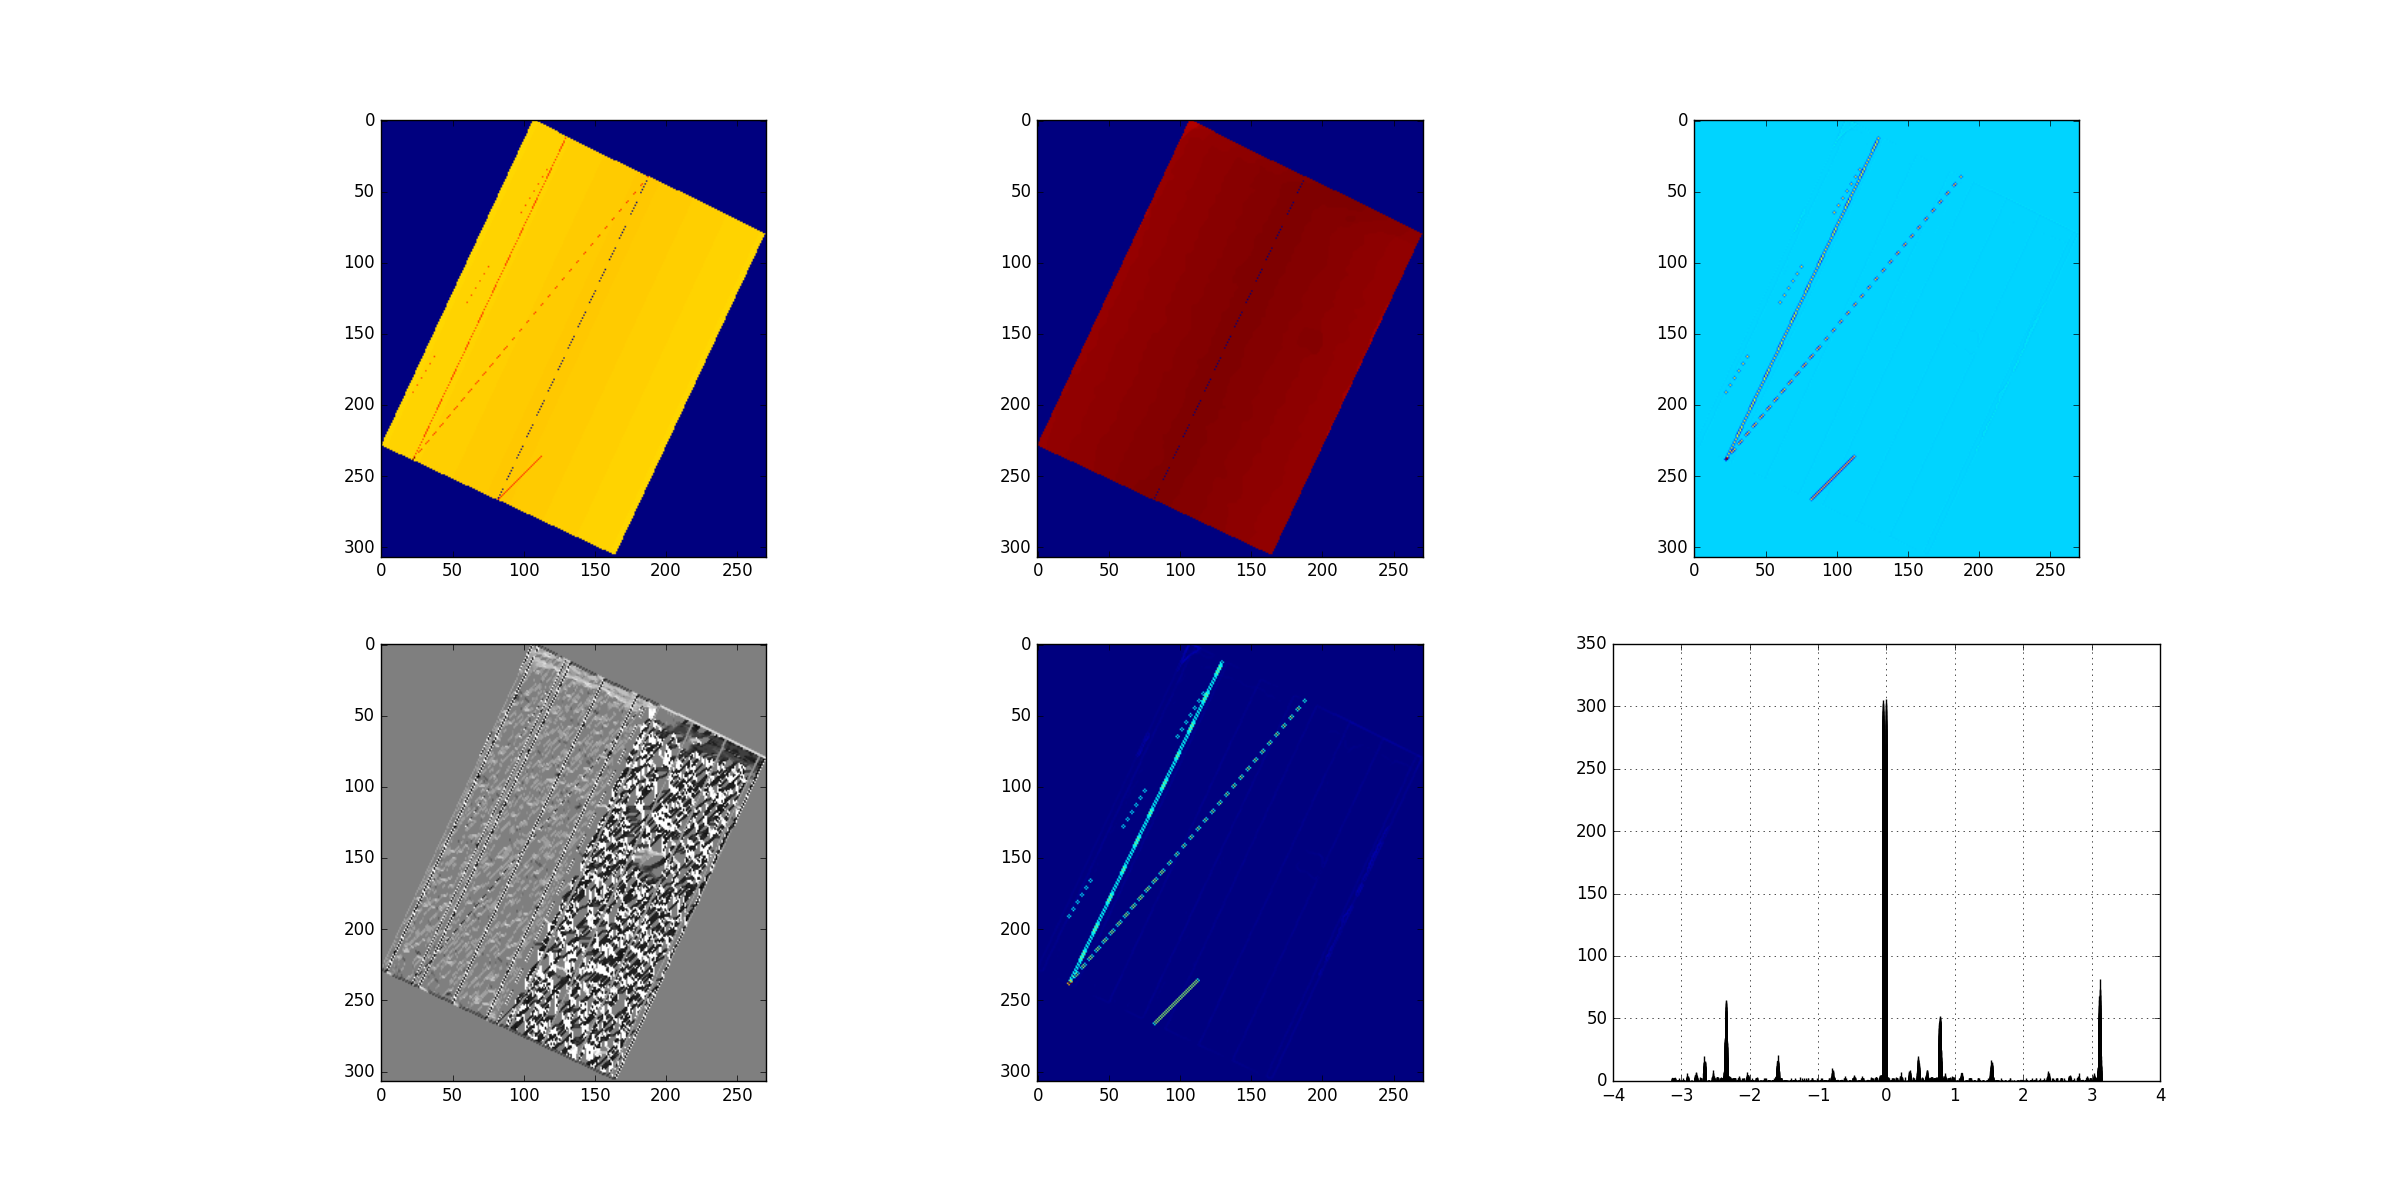
\includegraphics[scale=.25]{images/raster/elancourt/prototyping_1246-13704_T23621_T23622.png}
		\end{center}
	\end{figure}
	
\section*{Attachments:}

\begin{itemize}
	\item[-] You can checkout the Code in \href{https://github.com/Ethiy/3DSceneModel}{Github}.
	\item[-] You can also check the \href{https://github.com/Ethiy/3DSceneModel/projects/1}{dev kaban}.
\end{itemize}
	
\end{document}
